\documentclass[xcolor=table,handout]{beamer}
\setbeamertemplate{navigation symbols}{}

\usepackage{pgfpages}
\usepackage{adjustbox}
\setbeameroption{show notes}
\setbeameroption{show notes on second screen=right}

\usepackage{booktabs}
\usepackage{beamerthemeshadow}
\setbeamertemplate{caption}[numbered]
\setbeamerfont{caption}{size=\tiny}

% This week we will start a fun two-week Journal Club assignment. I've selected a set of articles on topics in Global Change science that have relied on remote sensing. This is a group project so the class will be grouped (~5 students) to cover a single topic.  See below how to start the grouping process. For the next 2 weeks ( with the break in between), I'd like each group to work together to read the articles and discuss them (you can have group discussions using the Groups area of Blackboard) or use the tab I have set in the Discussion area for Unit 10.  Then, each group must work together to summarize their articles, provide critical analysis, and lead a discussion presentation of their topic (in the Discussion section). Each group will also provide a PowerPoint or pdf presentation of the material to the class via the Discussion board I have set up for each group in Week 12.
% 
% Guidelines for presentations
% I'd like each group to briefly summarize the "meat" of the papers emphasizing the problem being addressed, a basic description of methods, and the main result/contribution. I'd also like to see the linkages between the papers discussed - how one result builds (or contradicts) earlier results. Finally, I'd like a critique of the papers (or each paper individually)... are there any weak points in the analyses? What could be done better in the future with improved technology? Obviously we aren't experts in all of these fields, but evaluating scientific findings is a common job in the policy arena, where many JHU grads end up working.  I suggest you get together in the Groups area (i.e., set up a forum for the group) and divide the work among the members.
% A PowerPoint or pdf slide presentation works best for conveying the asked for points of the articles along with some key supporting figures.  The format that seems to work well is:
% 
% Title Slide with author’s names and a cool cover image related to the topic
% 
% Introduction including background of the problem and topics covered by the articles
% 
% Summary of Articles: 1-2 slides for each article ( Title, Authors, Objectives, Methods, Findings, at least one informative image or graph
% 
% Overall Summary and Conclusion
% 
% Try to keep your presentations to 10-12 slides.
% 
% Grading
% Full credit for a student member of a journal club is awarded based on the quality of the presentation (10 points), contribution to the group (10 points).  In addition there will be a related Discussion during Unit 12 worth (5 points).  In order to assess a student’s participation and contribution to the presentation I ask that each group work in the designated Groups area.  This is separate from the class discussion forum that I will create for each group.
% 
% If you have any questions, post them in the Q/A section and send me an email.


\begin{document}

\title{Journal Club Presentation: Ocean Color}  
\author[K. Bellock, L. Chen, D. Durrance, A. Yen, H. Perez]{Kenneth Bellock, Leshi Chen, Danielle Durrance, Andrew Yen, Hack Perez}
\titlegraphic{%
    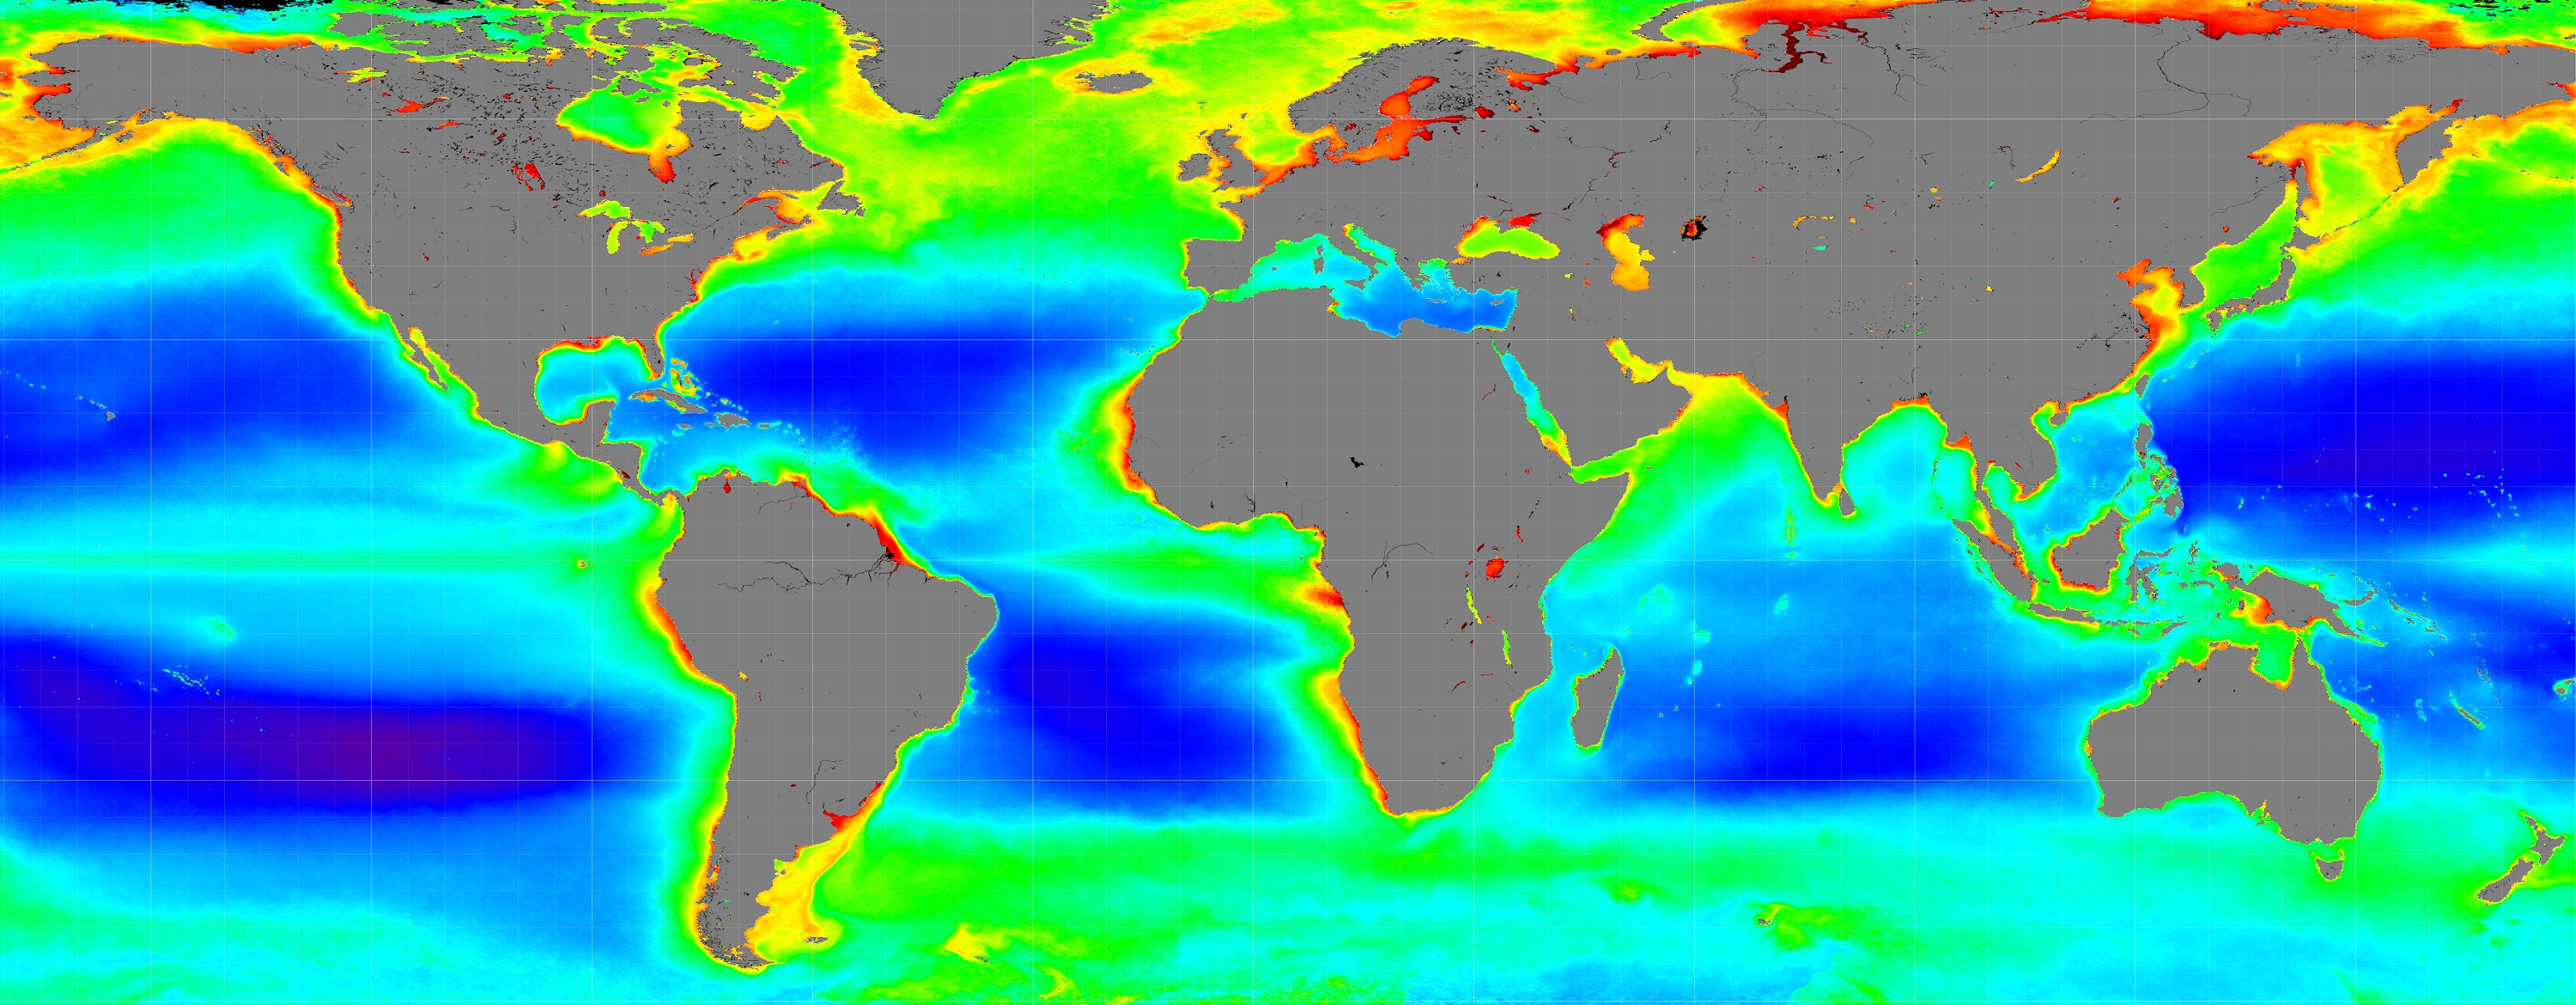
\includegraphics[height=.37\textheight]{15_037}

    \tiny \textbf{Source:} \url{https://www.nasa.gov/press/2015/march/new-nasa-mission-to-study-ocean-color-airborne-particles-and-clouds}
}
\date{\vspace*{-2.5em}\par April 4, 2018} 

\section{Introduction}

\begin{frame}
  \titlepage{}
  \note{Assumptions:}
  \note[item]{TODO:\@ List assumptions.}
\end{frame}

\begin{frame}\frametitle{Table of contents}
  \tableofcontents{}
  \note[item]{A road map is a great thing to have.}
  \note[item]{A joke or reference to current events in common culture would be great here if the audience appears receptive.}
\end{frame} 

\begin{frame}\frametitle{Introduction} 

  \note[item]{TODO:\@ Write Introduction}
\end{frame}

\section{Article Summaries}

\begin{frame}\frametitle{Paper 1} 

  \note[item]{TODO:\@ Include title, authors, objectives, methods, findings, and at least one informative image or graph.}
\end{frame}

\begin{frame}\frametitle{Paper 2} 

  \note[item]{TODO:\@ Include title, authors, objectives, methods, findings, and at least one informative image or graph.}
\end{frame}

\begin{frame}\frametitle{Paper 3} 

  \note[item]{TODO:\@ Include title, authors, objectives, methods, findings, and at least one informative image or graph.}
\end{frame}

\begin{frame}\frametitle{Paper 4} 

  \note[item]{TODO:\@ Include title, authors, objectives, methods, findings, and at least one informative image or graph.}
\end{frame}

\section{Summary and Conclusion}

\begin{frame}\frametitle{Summary} 

  \note[item]{TODO:\@ Write Summary}
\end{frame}

\begin{frame}\frametitle{Conclusion} 

  \note[item]{TODO:\@ Write Conclusion}
\end{frame}

\end{document}
